 \documentclass{beamer}
\mode<presentation>
\usepackage{amsmath}
\usepackage{amssymb}
%\usepackage{advdate}
\usepackage{graphicx}
\usepackage{adjustbox}
\usepackage{subcaption}
\usepackage{enumitem}
\usepackage{multicol}
\usepackage{mathtools}
\usepackage{listings}
\usepackage{url}
\def\UrlBreaks{\do\/\do-}
\usetheme{Boadilla}
\usecolortheme{lily}
\let\vec\mathbf
\setbeamertemplate{footline}
{
  \leavevmode%
  \hbox{%
  \begin{beamercolorbox}[wd=\paperwidth,ht=2.25ex,dp=1ex,right]{author in head/foot}%
    \insertframenumber{} / \inserttotalframenumber\hspace*{2ex} 
  \end{beamercolorbox}}%
  \vskip0pt%
}
\setbeamertemplate{navigation symbols}{}

\providecommand{\nCr}[2]{\,^{#1}C_{#2}} % nCr
\providecommand{\nPr}[2]{\,^{#1}P_{#2}} % nPr
\providecommand{\mbf}{\mathbf}
\providecommand{\pr}[1]{\ensuremath{\Pr\left(#1\right)}}
\providecommand{\qfunc}[1]{\ensuremath{Q\left(#1\right)}}
\providecommand{\sbrak}[1]{\ensuremath{{}\left[#1\right]}}
\providecommand{\lsbrak}[1]{\ensuremath{{}\left[#1\right.}}
\providecommand{\rsbrak}[1]{\ensuremath{{}\left.#1\right]}}
\providecommand{\brak}[1]{\ensuremath{\left(#1\right)}}
\providecommand{\lbrak}[1]{\ensuremath{\left(#1\right.}}
\providecommand{\rbrak}[1]{\ensuremath{\left.#1\right)}}
\providecommand{\cbrak}[1]{\ensuremath{\left\{#1\right\}}}
\providecommand{\lcbrak}[1]{\ensuremath{\left\{#1\right.}}
\providecommand{\rcbrak}[1]{\ensuremath{\left.#1\right\}}}
\theoremstyle{remark}
\newtheorem{rem}{Remark}
\newcommand{\sgn}{\mathop{\mathrm{sgn}}}
\providecommand{\abs}[1]{\vert#1\vert}
\providecommand{\res}[1]{\Res\displaylimits_{#1}} 
\providecommand{\norm}[1]{\lVert#1\rVert}
\providecommand{\mtx}[1]{\mathbf{#1}}
\providecommand{\mean}[1]{E[ #1 ]}
\providecommand{\fourier}{\overset{\mathcal{F}}{ \rightleftharpoons}}
%\providecommand{\hilbert}{\overset{\mathcal{H}}{ \rightleftharpoons}}
\providecommand{\system}[1]{\overset{\mathcal{#1}}{ \longleftrightarrow}}
%\providecommand{\system}{\overset{\mathcal{H}}{ \longleftrightarrow}}
	%\newcommand{\solution}[2]{\vec{Solution:}{#1}}
%\newcommand{\solution}{\noindent \vec{Solution: }}
\providecommand{\dec}[2]{\ensuremath{\overset{#1}{\underset{#2}{\gtrless}}}}
\newcommand{\myvec}[1]{\ensuremath{\begin{pmatrix}#1\end{pmatrix}}}


\lstset{
%language=C,
frame=single, 
breaklines=true,
columns=fullflexible
}
\lstset{
  language=C,
  basicstyle=\ttfamily\footnotesize,
  keywordstyle=\color{blue}\bfseries,
  commentstyle=\color{gray}\itshape,
  stringstyle=\color{orange},
  numbers=left,
  numberstyle=\tiny\color{gray},
  breaklines=true,
  frame=single,
  showstringspaces=false,
  tabsize=4,
  captionpos=b
}
\numberwithin{equation}{section}
\lstset{
  language=Python,
  basicstyle=\ttfamily\small,
  keywordstyle=\color{blue},
  stringstyle=\color{orange},
  numbers=left,
  numberstyle=\tiny\color{gray},
  breaklines=true,
  showstringspaces=false
}

\title{Problem 4.4.31}
\author{Sujal Rajani}

\date{\today} 
\begin{document}

\begin{frame}
\titlepage
\end{frame}

\section{Question}
\begin{frame}{Question}
\textbf{QUESTION}
\\
Find the equation of the line joining $\vec{A}$(1,3) and $\vec{B}$ (0,0).Also,find k if $\vec{D}$ (k,0) is a point such that the area of $\triangle ABD$ is 3 square units.
\end{frame}
\begin{frame}{Solution}
\textbf{SOLUTION}
as mentioned in the problem the position vector of the points is :
\\
\begin{align*}
    \vec{A}=\myvec{1\\3},\vec{B}=\myvec{0\\0},\vec{D}=\myvec{k\\0}
\end{align*}
the general equation of a line passing through two position vector $\vec{B}$ and $\vec{A}$ is :
\begin{align*}
    \vec{L}=\vec{H}+z\myvec{1\\m}
\end{align*}
$\vec{H}$:is either the position vector of $\vec{A}$ OR $\vec{B}$
\\
m is the slope of the line .

 \end{frame}
\begin{frame}{Solution}
\begin{align*}
    m=\dfrac{y_2-y_1}{x_2-x_1}
    \\
    \vec{A}=\myvec{x_2\\y_2},\vec{B}=\myvec{x_1\\y_1}
    \\
    m=3
\end{align*}

\\
z is an arbitrary constant .
\\
the equation of line passing through  $\vec{B}$ and $\vec{A}$ is :
\\
\begin{align*}
    \vec{L}=\myvec{0\\0}+z\myvec{1\\3}
\end{align*}
area of $\triangle ABD $ : 
\\
\begin{align*}
    \dfrac{1}{2}||(\vec{A}- \vec{B})X(\vec{D}- \vec{B})||=3
\end{align*}
     \end{frame}
     \begin{frame}{VECTOR PRODUCT}
     \textbf{VECTOR PRODUCT}
\\
let N be a vector :
\begin{align}
    \vec{N}=\myvec{n_1\\n_2\\0}
    \\
    \end{align}
    let M be a vector :
    \begin{align}
    \vec{M}=\myvec{m_1\\m_2\\0}
\end{align}
the vector product of two vectors $\vec{N}$ and $\vec{M}$ is 
\\
\vec{N}X\vec{M} =
\myvec{
n_{23} & m_{23} \\
n_{31} & m_{31} \\
n_{12} & m_{12}
}
=
\myvec{
n_2 m_3 - n_3 m_2 \\
n_3 m_1 - n_1 m_3 \\
n_1 m_2 - n_2 m_1
}
=
\myvec{
3 \times 0 - 0 \times 0 \\
0 \times k - 1 \times 0 \\
1 \times 0 - 3 \times k
}
=
\myvec{
0 \\
0 \\
3k
}
\end{frame}
     \begin{frame}{solution}
         {area of $\triangle ABD$ is :}
\begin{align*}
    \dfrac{1}{2}||(\vec{A}-  \vec{B})X(\vec{D} -  \vec{B})||=\dfrac{1}{2}||\myvec{1\\3\\0}X\myvec{
    K\\0\\0}||= \dfrac{1}{2}\sqrt{\myvec{0\\0\\3K}^\top\myvec{0\\0\\3K}}=3
    \end{align*}
    \begin{align*}
        k=+2,-2
    \end{align*}
    n1=1,n2=3,m1=k,m2=0
\\
for the conveniences we are taking  $\vec{D_1}$and $\vec{D_2}$
\\
    so the position vector of $\vec{D}$ :
    \begin{align*}
        \vec{D_1}=\myvec{2\\0},\vec{D_2}=\myvec{-2\\0}
    \end{align*}
     \end{frame}
       \begin{frame}[fragile]
    \begin{figure}[H]
    \centering
    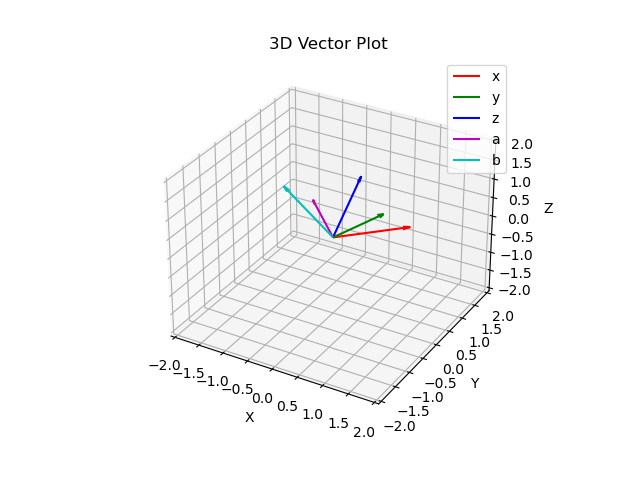
\includegraphics[width = 0.6\columnwidth]{../figs/img.png}
    \caption*{}
    \label{figs}
\end{figure}
\end{frame}
\section{ C Code}
\begin{frame}[fragile]
\frametitle{C Code }
\begin{lstlisting}[language=C]
#include <stdio.h>
#include <stdlib.h>
#include <math.h>

int main() {
    // Coordinates for A, B
    int x1 = 1, y1 = 3;
    int x2 = 0, y2 = 0;

    // Calculate slope and intercept
    float m = (float)(y2 - y1) / (x2 - x1); // Slope
    float c = y1 - m * x1; // Intercept
    printf("Equation of line AB: y = %.2fx + %.2f\n", m, c);
\end{lstlisting}
\end{frame}

\begin{frame}[fragile]
\frametitle{C Code }
\begin{lstlisting}[language=C]
        // Area of triangle formula in coordinates:
    // Area = (1/2) * |x1(y2-y3) + x2(y3-y1) + x3(y1-y2)|
    // Let D(k,0) = (x3, y3)
    int y3 = 0;
    float area_target = 3.0;
    // Substitute:
    // area = 0.5 * |1*(0-0) + 0*(0-3) + k*(3-0)|
    //       = 0.5 * |3*k|
    // Set 0.5 * |3*k| = 3  => |k| = 2
    float k1 = 2.0, k2 = -2.0;

    printf("Possible values of k for D(k,0): %.2f and %.2f\n", k1, k2);

    return 0;
}
\end{lstlisting}
\end{frame}
\begin{frame}[fragile]
\frametitle{Python Code for Plotting}
\begin{lstlisting}[language=Python]
import numpy as np
import matplotlib.pyplot as plt
from line.funcs import *
# from triangle.funcs import *
# from conics.funcs import circ_gen
# if using termux
import subprocess
import shlex
# end if

\end{lstlisting}

\end{frame}

\begin{frame}[fragile]
\frametitle{Python Code for Plotting}
\begin{lstlisting}[language=Python]
# Triangle vertices
A = np.array([1,3]).reshape(-1,1)
B = np.array([0,0]).reshape(-1,1)
D = np.array([2,0]).reshape(-1,1)
D' = np.array([-2,0]).reshape(-1,1
coords = np.block([[A,B,D,D']])
# Generate triangle sides
AB = line_gen(A,B)
BD = line_gen(B,D)
DA = line_gen(D,A)
BD' = line_gen(B,D')
D'A = line_gen(D',A)
\end{lstlisting}

\end{frame}
\begin{frame}[fragile]
\frametitle{Python Code for Plotting}
\begin{lstlisting}[language=Python]


# Plot sides
plt.plot(AB[0,:],AB[1,:], label='AB')
plt.plot(BD[0,:],BD[1,:], label='BD')
plt.plot(DA[0,:],DA[1,:], label='DA')
plt.plot(BD'[0,:],BD'[1,:], label='BD'')
plt.plot(D'A[0,:],D'A[1,:], label='D'A)
\end{lstlisting}

\end{frame}
\begin{frame}[fragile]
\frametitle{Python Code for Plotting}
\begin{lstlisting}[language=Python]
# Scatter vertices
plt.scatter(coords[0,:],coords[1,:])
plt.text(A[0],A[1],"A(1,3)")
plt.text(B[0],B[1],"B(0,0)")
plt.text(D[0],D[1],"D(2,0)")
plt.text(D'[0],D'[1],"D'(-2,0)")
# Styling
plt.xlabel('$x$')
plt.ylabel('$y$')
plt.legend(loc='best')
plt.grid(True)
plt.axis('equal')

plt.savefig('../figs/triangle.png')
plt.show()

\end{lstlisting}

\end{frame}
\end{document}